% !TeX spellcheck = fr_FR

% TODO: Replace scan images with clean text where possible

\documentclass[a4paper, 10pt]{report}

\usepackage[french]{babel}
\usepackage[T1]{fontenc}

\usepackage{amsmath, amssymb, amsfonts}

\usepackage{hyperref}
\usepackage{geometry}

\usepackage{xcolor}
\usepackage{graphicx}

\usepackage{fancyhdr}
\usepackage{lastpage}

\usepackage{enumitem}

\geometry{
	a4paper,
	left=25mm,
	right=25mm,
	top=35mm,
	bottom=25mm,
	headsep=5mm,
	headheight=20mm,
}

\definecolor{solution}{HTML}{E5E4E2}
\providecommand{\abs}[1]{\lvert#1\rvert}
\providecommand{\norm}[1]{\lVert#1\rVert}
\DeclareMathOperator{\card}{card}

\makeatletter
\renewcommand*\env@matrix[1][*\c@MaxMatrixCols c]{%
	\hskip -\arraycolsep
	\let\@ifnextchar\new@ifnextchar
	\array{#1}}
\makeatother

\begin{document}
	
	\renewcommand{\headrule}{%
		\vspace{-4pt}\hrulefill
		\raisebox{-6.8pt}{\ 
\includegraphics[height=5mm]{../../icon.png}}
		\hrulefill
	}	
	\pagestyle{fancy}
	\fancyhf{}
	
	\fancyhead[L]{\small \slshape Automne 2024}
	\fancyhead[C]{\Large \bfseries Algèbre I - Série 08}
	\fancyhead[R]{\small Buff Mathias}
	\fancyfoot[L]{
		\small Source files available at:
		\href{https://github.com/MathiasBuff/bsc-math}
		{github.com/MathiasBuff/bsc-math}
	}
	\fancyfoot[R]{
		\small Page \thepage
		\hspace{1pt} /
		\pageref*{LastPage}
	}
	

	\noindent
	\textbf{Exercice 1.}\\
	On considère $\mathcal{B} = \{(2, 1), (5, 3)\}$ une base de
	$\mathbb{R}^2$ et $\mathcal{C} = \{(1, 0, 1), (1, 1, 0), (1, 1, 1)\}$
	une base de $\mathbb{R}^3$. Soit $f: \mathbb{R}^2 \to \mathbb{R}^3$.
	l'application linéaire dont la matrice relativement aux bases
	$\mathcal{B}$ et $\mathcal{C}$ est donnée par
	\[
		M_{\mathcal{C},\mathcal{B}}(f) =
		\begin{pmatrix}
			7 & -3\\
			2 & 1\\
			8 & 0\\
		\end{pmatrix}
	\]
	Trouver la matrice $M_{\mathcal{E}',\mathcal{E}}(f)$ où
	$\mathcal{E}, \mathcal{E}'$ sont les bases canoniques de
	$\mathbb{R}^2$ et $\mathbb{R}^3$ respectivement.

	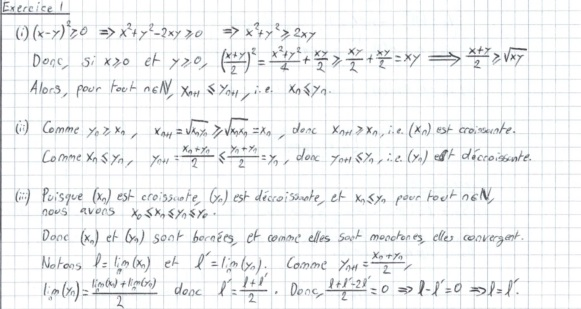
\includegraphics{ex01.jpg}

	\vspace{5mm}
	\noindent
	\textbf{Exercice 2.}\\
	Soient $\mathcal{E}_1 = \{v_1, v_2, v_3\}, \mathcal{B}_1 =
		\{5v_1 - 3v_2 + 2v_3, v_1 + 2v_2 - v_3, v_1 + v_2 + v_3\}$ deux
	bases de $\mathbb{R}^3$ et\\
	$\mathcal{E}_2 = \{w_1, e_2\}, \mathcal{B}_2 =
		\{w_1 + 2w_2, -w_1 - w_2\}$ deux bases de $\mathbb{R}^2$.
	Soit $f: \mathbb{R}^3 \to \mathbb{R}^2$ l'application linéaire dont
	la matrice relativement aux bases $\mathcal{E}_1$ et $\mathcal{E}_2$
	est donnée par
	\[
		M_{\mathcal{E}_2,\mathcal{E}_1}(f) =
		\begin{pmatrix}
			3 & -1 & 2\\
			4 & 1 & -3\\
		\end{pmatrix}
	\]
	Déterminer $M_{\mathcal{B}_2,\mathcal{B}_1}(f)$.
	
	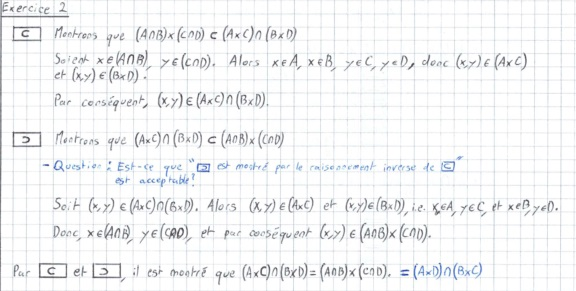
\includegraphics{ex02.jpg}
	
	\newpage
	
	\fancyhf{}
	\renewcommand{\headrule}
	{\rule{\textwidth}{0pt}}
	\fancyfoot[R]{
		\small Page \thepage
		\hspace{1pt} /
		\pageref*{LastPage}
	}
	
	\noindent
	\textbf{Exercice 3.}
	\begin{enumerate}[label=\arabic*., leftmargin=7mm]
		\item Soit $\sigma$ la permutation de $\{1, 2, 3, 4, 5, 6, 7, 8\}$
		définie par \[\sigma(1) = 7, \quad \sigma(2) = 5, \quad
		\sigma(3) = 3, \quad \sigma(4) = 1, \quad \sigma(5) = 2, \quad
		\sigma(6) = 4, \quad \sigma(7) = 6, \quad \sigma(8) = 8.\]
		Écrire la décomposition de $\sigma$ en produit de cycles
		et une décomposition de $\sigma$ en produit de\\ transpositions.
		%
		\item Écrire la décomposition en cycles du produit des permutations
		(1 2 3)(2 3 4) dans le groupe\\ symétrique $S_n$, où $n$ est un
		entier, $n \geq 4$.
		%
		\item Calculer la signature de la permutation $\sigma \in S_5$
		définie par\\ $\sigma(1) = 4, \quad \sigma(2) = 1, \quad
		\sigma(3) = 5, \quad \sigma(4) = 3, \quad \sigma(5) = 2.$
		%
		\item Calculer la signature de la permutation $\sigma \in S_n$
		définie par $\sigma = (1 2 \dotso k)$ (cycle de longueur $k$).
	\end{enumerate}
	
	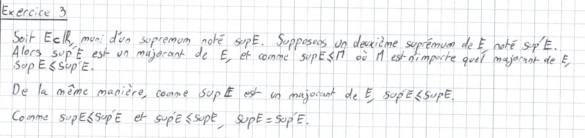
\includegraphics{ex03.jpg}
	
	\vspace{5mm}
	\noindent
	\textbf{Exercice 4.}\\
	Soit $\sigma \in S_5$ la permutation définie par $\sigma(1) = 2,
		\quad \sigma(2) = 1, \quad \sigma(3) = 4, \quad \sigma(4) = 5,
		\quad \sigma(5) = 3$. Quel est le plus petit entier $k \geq 1$
	pour que $\sigma^k$ (la composée $k$ fois de $\sigma$) soit l'identité ?
	
	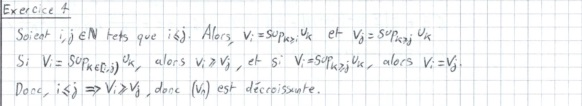
\includegraphics{ex04.jpg}
	
	\vspace{5mm}
	\noindent
	\textbf{Exercice 5.}\\
	Soient $A \in \mathcal{M}_{n, n}(\mathbb{K})$ et
	$\lambda \in \mathbb{K}$. Montrer que $\mathrm{det}(\lambda A)
		= \lambda^n \mathrm{det}(A)$.
		
	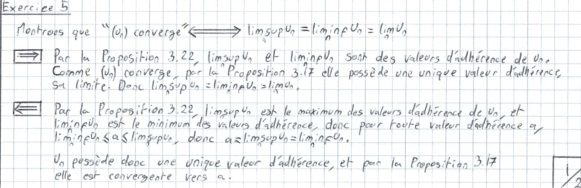
\includegraphics{ex05.jpg}
	
	\newpage
	
	\noindent
	\textbf{Exercice 6.}\\
	Soit $A \in \mathcal{M}_{n, n}(\mathbb{C})$. Montrer que
	$\mathrm{det}(\overline{A}) = \overline{\mathrm{det}({A})}$, où
	$\overline{A}$ est la matrice conjuguée complexe définie par
	$\overline{A} = (\overline{a_{ij}})_{i, j = 1, \dotsc, n}$.
	
	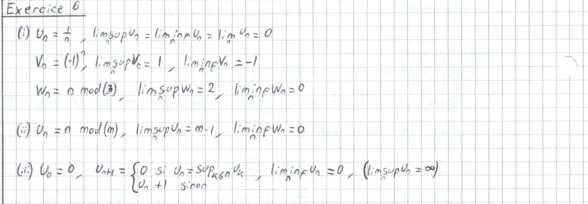
\includegraphics{ex06.jpg}
	
	\vspace{5mm}
	\noindent
	\textbf{Exercice 7.}\\
	Soit $A \in \mathcal{M}_{n, n}(\mathbb{K})$.
	\begin{enumerate}[label=\arabic*., leftmargin=7mm]
		\item Montrer que le rang de $A$ est égal au nombre maximal
		de colonnes linéairement indépendantes de $A$.
		%
		\item Montrer que le rang de $A$ est égal au nombre maximal
		de lignes linéairement indépendantes de $A$.
		%
		\item Montrer que le rang de $A$ est égal au nombre de pivots
		de la matrice $A$ (Indication : regarder l'effet des opérations
		élémentaires de la méthode du pivot sur le rang).
	\end{enumerate}
	
	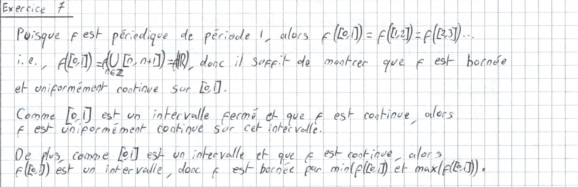
\includegraphics{ex07.jpg}

	
%	
%	\colorbox{solution}
%	{
%		\begin{minipage}{0.9\textwidth}
%			s
%		\end{minipage}
%	}
%	
%	\colorbox{solution}
%	{
%		\begin{minipage}{0.9\textwidth}
%			\begin{enumerate}[label=(\alph*)]
%				\item a
%			\end{enumerate}
%		\end{minipage}
%	}
	
\end{document}
